\documentclass[a4paper, 12pt]{report}

% Charset
\usepackage[utf8]{inputenc}
% Language
\usepackage[british]{babel}
% Font
\usepackage[default]{sourcesanspro}
\usepackage[T1]{fontenc}
\usepackage{titlesec, color}
\definecolor{gray75}{gray}{0.75}
\newcommand{\hsp}{\hspace{20pt}}
\usepackage{microtype}
% Color
\usepackage{xcolor}
% Graphics
\usepackage{graphicx}
\usepackage{fancyhdr}
\graphicspath{ {./img/} }
% Indexing
\usepackage{index}
\makeindex
% Hyperlinks
\usepackage{hyperref}
\hypersetup{
 	colorlinks=true, 
	linkcolor=black,
	urlcolor=blue,
}

\begin{document}

% Title page
\title{\Large{\textbf{The Bitcoin Lightning Network}}}
\author{Yannick Mawuena Rüfenacht \\ \href{mailto:yannick.ruefenacht@hotmail.com}{yannick.ruefenacht@hotmail.com}}
\date{October 21, 2020\\Version 1.0.0}
\maketitle

% Quote
\begin{quote}
\vspace*{\fill}
\textit{``Lightning is a decentralized network using smart contract functionality in the blockchain to enable instant payments across a network of participants."}
\par\raggedleft--- \textup{Joseph Poon}
\vspace*{\fill}
\end{quote}

% Abstract
\begin{abstract}
Today’s Bitcoin protocol provides the possibility to participate in a secure decentralized payment system without a single custodial third-party holding funds. This system uses the blockchain technology to distribute all performed transactions across the network of participants for them to reach general consensus. The process of securing and distributing transactions takes up a substantial amount of time, which creates a significant drag on the ability to encompass all global financial transactions. The idea of the lightning network is to create micropayment channels between participants that operate off-blockchain. These channels can be used to instantly exchange Bitcoins without distributing them to the blockchain. Upon closing a micropayment channel, the final balance of that channel is broadcasted to the main blockchain. This concept could prove to be useful especially in situations where two participants frequently exchange money.
\end{abstract}

% Table of Contents
\tableofcontents
\listoffigures

% Formatting
\setlength{\parskip}{1em}
\setlength{\parindent}{0em}
\titleformat{\chapter}[hang]{\LARGE\bfseries}{\thechapter\hsp\textcolor{gray75}{|}\hsp}{0pt}{\LARGE\bfseries}
\titleformat{\section}[hang]{\large\bfseries}{\thesection\hsp\textcolor{gray75}{|}\hsp}{0pt}{\large\bfseries}

\widowpenalties 1 10000
\raggedbottom

\chapter{Introduction}
\par The primary aim of this paper is to provide a simple to understand explanation of the Lightning Network and why it is necessary. Furthermore, this paper also dives into the underlying system upon which the Lightning Network operates, namely the Bitcoin blockchain system. The Lightning Network uses the blockchain and Bitcoin smart contracts to create a secure network of participants which are able to perform transactions at high volume and speed. To be able to understand how the lightning network works or why it is even necessary, requires a basic understanding of the blockchain and Bitcoin.
\par This paper guides the reader through a list of steps that show how the lightning network is built, starting from the basics of a blockchain. Each step builds on top of the previous one. It is therefore recommended to read this paper in the right order.

\chapter{A Brief Overview of the Bitcoin Blockchain}
\par The way of ordinary banking systems usually goes as follows: The customer deposits his money on a bank account and when a payment is done, the bank either adds or subtracts the amount from his or her account. Or sometimes the customer withdraws some money from the ATM. The underlying concern hereby is that in each of those use cases there is always one centralized system involved which is in power of handling all the transactions. The inner workings of that system are strictly sealed to the outside, which has the capability to create trust issues. And this is where the idea of Bitcoin comes to the surface.

\section{The Idea of Bitcoin}
\par The main idea of Bitcoin is to remove the aspect of centralized control and to form a network of users where everyone is connected to everyone and the same rights apply to everyone.  

\begin{figure}[h]
	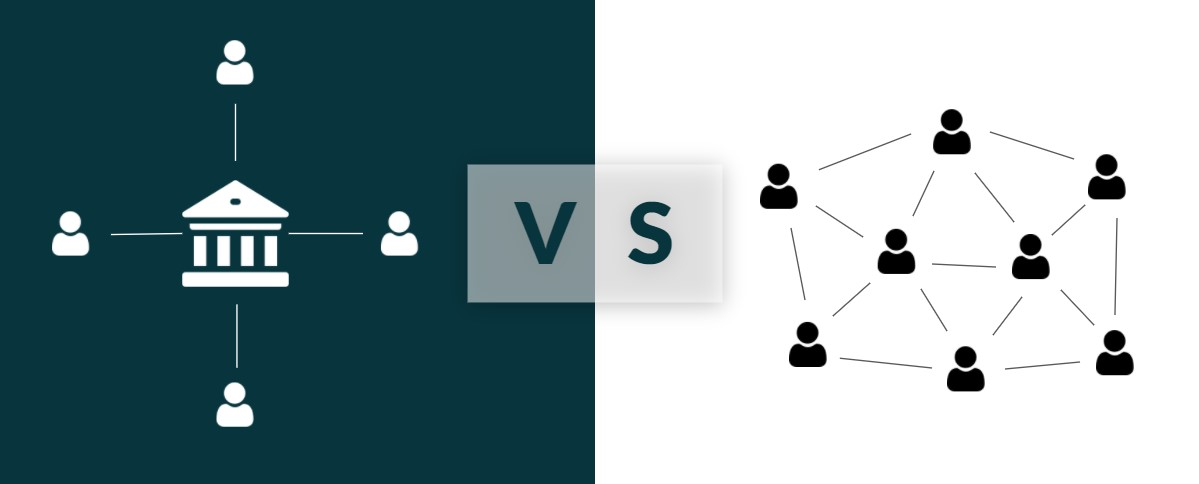
\includegraphics[width=\textwidth]{01_Decentralized}
	\caption{Conventional Banking System vs Decentralized System}
	\label{fig:01_Decentralized}
\end{figure}

\par To achieve this, the history of all transactions is stored in a public ledger, which is accessible to everyone. But instead of storing this ledger in one central place, every participant obtains their own copy so that the ledger is distributed to everyone throughout the network of participants. Anyone who then performs a transaction broadcasts it out to the entire world for everyone to hear and to include it in their private ledgers. 
\par At first, the degree of openness that this system provides might seem absurd. But the fact that all the records of the transactions are publicly available also means that everyone can verify the validity of every transaction. And this is where Bitcoin gains its immense trust and security benefits.

\section{The Issue of Decentralization}
\par Although the approach of a centralized network seems quite appealing so far, there is an important issue that arises very quickly. While the idea of everyone broadcasting their transactions to the entire network would work for a small number of people, it would become significantly more difficult to ensure that every member of the network receives every transaction in the same order, as the number of participants increases. Network delays could cause transactions to arrive in different orders in different places. This raises the question: How can the ledger maintain the right order of transactions across the entire network of participants. 
\par This is precisely the problem that was addressed in the original Bitcoin paper. The solution that Bitcoin offers lies within the functionality of its blockchain.

\section{The Bitcoin Blockchain}
\par In order to maintain the right order of all transactions, the broadcasting of new transactions needs to be regulated and a new mechanism that locks the order off all the transactions needs to be implemented.
\paragraph{Blocks} \hspace{0pt} \\
First of all, the ledger is split into a group of blocks. Each block contains a set of transactions and a special value at the bottom that is referred to as the “proof of work”. 

\begin{figure}[h]
	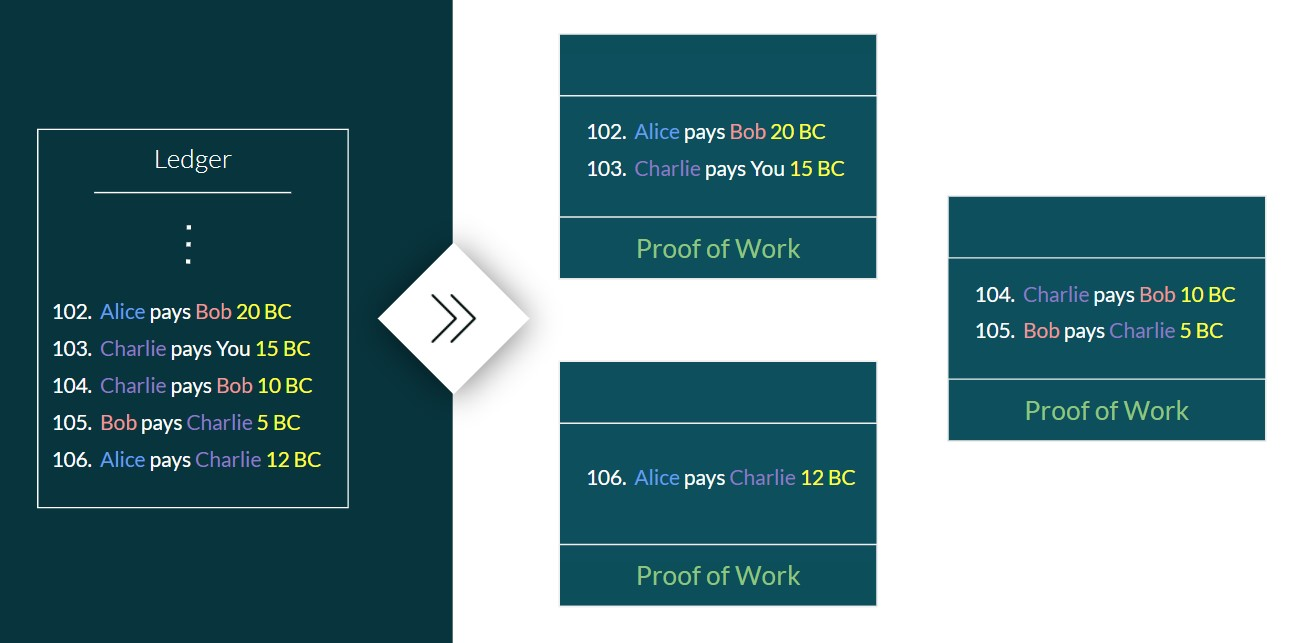
\includegraphics[width=\textwidth]{02_Ledger_Blocks}
	\caption{Ledger being split into blocks}
	\label{fig:02_Ledger_Blocks}
\end{figure}

\paragraph{Proof of work} \hspace{0pt} \\
The proof of work, also known as the hash of the block, is a special numeric value that is required for each block. A block without a proof of work is considered invalid. The value is special in the sense that it needs to be calculated. The calculation takes on average 10 minutes of computational work. This process is usually performed by special members of the network called “Minors”. The purpose of this mechanism is to regulate the number of transactions that are being broadcasted and to make it difficult for attackers to generate new blocks. Furthermore, the proof of work is unique for each block, this means that it could also act as a unique identifier.
\paragraph{Ordering transactions} \hspace{0pt} \\
To maintain a fixed order to these blocks, each block additionally contains the proof of work of its previous block.\footnote{The first block is a special case since it cannot point to a previous block. It is named the Genisis Block} This causes each block to have a reference to its previous block which ultimately results in a fixed list.

\begin{figure}[h]
	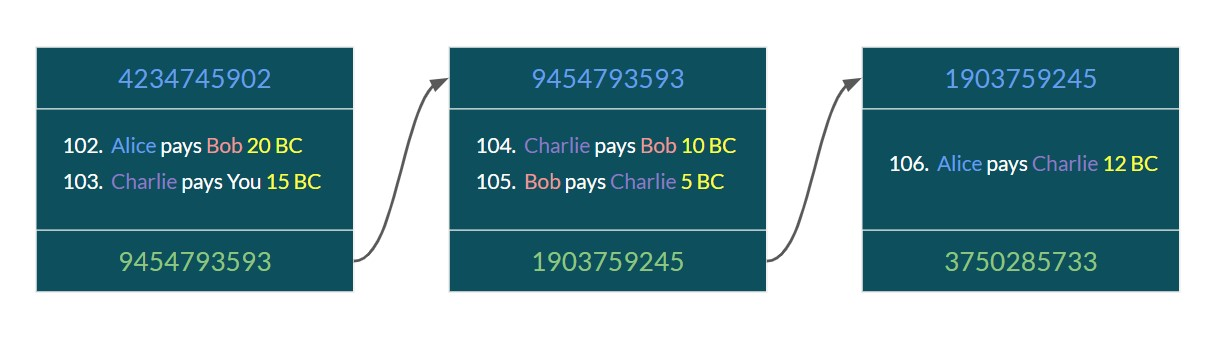
\includegraphics[width=\textwidth]{03_Linked_Blocks}
	\caption{Chaining of the blocks}
	\label{fig:03_Linked_Blocks}
\end{figure}

\paragraph{Security} \hspace{0pt} \\
The proof of work, or hash, is unique for each block as aforementioned. It is calculated using the contents of the block i.e., the set of transactions and the hash of the previous block. If the content gets changed, the hash automatically gets changed as well. The fact that each block contains the hash of the previous block is precisely what makes the blockchain so secure. 
\par If for example the content of the second block from the picture above gets tampered, it would automatically change its hash. This in turn would make the third block invalid since it no longer stores a valid hash of its previous block. Altering the third block causes the fourth block to be invalid. This scenario repeats itself throughout the entire list. This means that changing one block would consequently require changing the entire chain of blocks for it to be valid again. 
\par Since the ledger now basically consists of a group of blocks that are immutably chained together, it is commonly referred to as the “blockchain”. 

\section{The Ledger is the Currency}
\par Bitcoin is said to be a cryptocurrency. This poses the question: What actually is a cryptocurrency? The answer is quite simple: \textit{It is a ledger. The history of transactions is the currency.}
\par That being said, it is theoretically possible to remove the need for cash. Hypothetically, if everyone in the world used this ledger, it would be possible to send and receive money on this ledger for all eternity without ever converting it to cash.

\chapter{The Scalability Problem with Bitcoin}
\par As far as safety is concerned, Bitcoin provides an excellent solution with its use of a distributed ledger. The Bitcoin blockchain requires, that all state modifications of the ledger must be broadcasted to each node of the Bitcoin network. It is through this mechanism that a general consensus of everyone’s balances can be achieved. However, as a payment platform, Bitcoin by itself cannot handle the whole transactions of the world anytime in the near future. The fact that all transactions must be broadcasted throughout the entire world, creates significant time delays which result in Bitcoin being only able to handle a few transactions per second.

\chapter{Introducing the Lightning Network}
\par The Lightning network presents an additional layer that operates on top of the Bitcoin blockchain with the aim to enable instant and feeless micropayments. It has been introduced in 2015 and has been in development ever since. The main idea of the Lightning Network is to establish separate end-to-end connections between participants in order to not store every small transaction on the main blockchain, but rather off-blockchain. These connections are named micropayment channels or simply payment channels.

\section{Payment channels}
\par If two participants regularly exchange amounts, they would open a new payment channel between them, that is off-blockchain. This allows them to perform quick payments between each other. Once they conclude their business, they conduct a closing transaction on the main blockchain which contains the final balances of their wallets on the payment channel. That way, even if thousands of transactions are performed on the payment channel, only two transactions will be stored on the blockchain eventually. One for opening and one for closing the payment channel.

\paragraph{Creating a new payment channel} \hspace{0pt} \\
During the initiation of the payment channel, both parties provide a certain balance of Bitcoin onto their ends of the payment channel, allowing that balance to go back and forth between them whenever transactions are made. To complete the creation of the new payment channel, the inputs of both parties are put into a transaction that gets signed by both parties, and eventually, broadcasted on the main blockchain. This transaction is called the funding transaction.

\paragraph{Commitment transactions} \hspace{0pt} \\
Once the funding transaction has been added to the blockchain and settled, both parties can spend their balances on the channel in a series of commitment transactions that reallocate their balances accordingly. These kinds of transactions can remain between the channel participants and do not need to be stored on the blockchain.

\paragraph{Closing the payment channel} \hspace{0pt} \\
The balances of both parties can remain off-blockchain and be updated continuously until finally a settlement transaction is performed. This transaction contains the final balances of both parties and gets added to the main blockchain.

\paragraph{Examples} \hspace{0pt} \\
In the example money flows both ways in the payment channel, therefore it is considered a bi-directional payment channel.

\begin{figure}[h]
	\centering
	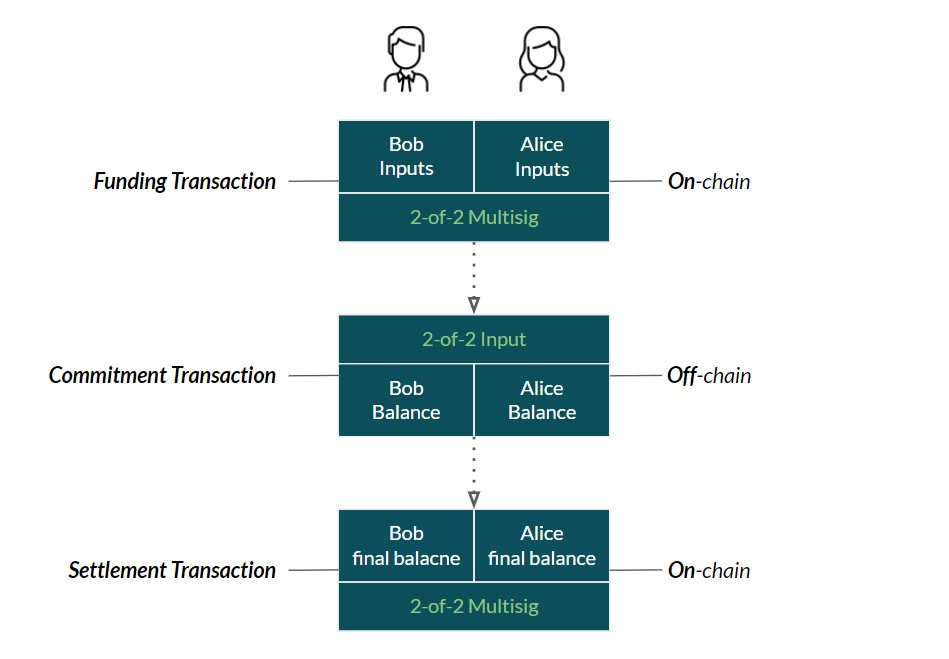
\includegraphics[width=13cm]{04_Bidirectional_Channel}
	\caption{Bi-directional payment channel}
	\label{fig:04_Bidirectional_Channel}
\end{figure}

\par Naturally, there can also be payment channels where money only flows in one direction, from one party to another. The example below demonstrates how a payment channel could be used to perform micropayments to an internet service provider in exchange for mobile data.

\begin{figure}[h]
	\centering
	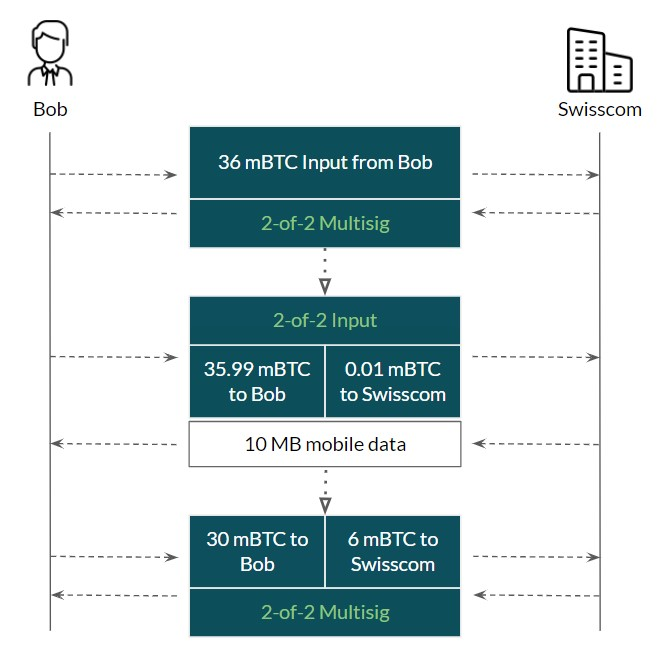
\includegraphics[width=10cm]{05_Onedirectional_Channel}
	\caption{Example of a payment channel to pay for mobile data usage}
	\label{fig:05_Onedirectional_Channel}
\end{figure}

\paragraph{Security} \hspace{0pt} \\
Payment channels rely on Bitcoin security primitives which prevent participants from stealing Bitcoin or losing Bitcoin due to uncooperative behaviour from the opposite party. Such security primitives include Multi-Signatures, Timelocks and No-Double-Spends.

\section{Multi-Signatures}
\par As the name suggests, the idea behind Multisig technology is to have multiple keys be in control of a Bitcoin balance. Multi-Signatures are described as K of N signature schemes, meaning that there are N valid predefined signatories that are authorized to release funds from a particular Bitcoin balance. Of those N keys, K is the number of signatures that are required to sign a transaction.

\paragraph{2 of 2 Multi-Signature} \hspace{0pt} \\
In the case of the Lightning Network, a 2 of 2 Multi-Signature type is used. This requires both parties of the channel to sign any transaction, because of that, one party alone cannot sign and execute a transaction on their own.

\section{Timelocks}
\par A payment channel gets closed when either party decides to publish the latest transaction onto the blockchain. That said, there is one major security concern about this idea. If for example Bob and Alice are using a payment channel in which, according to the latest commitment transaction, Alice has a greater Balance than Bob, the Question arises: Can Bob not simply broadcast a prior state in which he had a more advantageous balance and thus cheat?

\par The way this can be solved is to set a timelock. A timelock is an embedded delay or countdown in a commitment transaction that determines when the transaction becomes valid. Later commitment transactions have a shorter timelock and will therefore become valid sooner. This prevents either party from spending an older commitment transaction.

\begin{figure}[h]
	\centering
	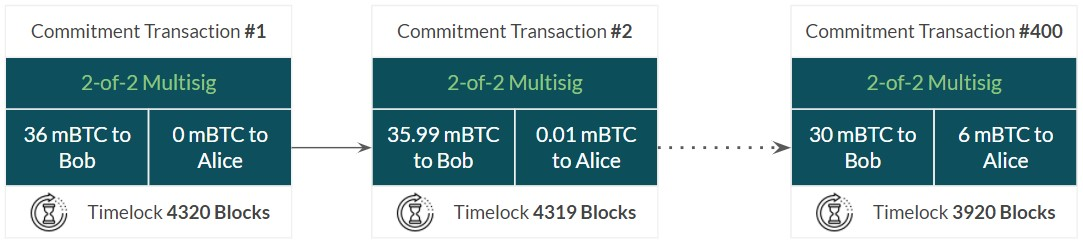
\includegraphics[width=13cm]{06_Timelocks}
	\caption{Transaction number 400 has the smallest timelock and thus becomes valid sooner than every other transaction}
	\label{fig:06_Timelocks}
\end{figure}

\section{No Double-Spend}
\par Once a commitment transaction has been broadcasted and its timelock has finished, it becomes a legitimate transaction and all the other commitment transactions automatically become invalid, since there can only be one final settlement transaction per payment channel. This principle is called No Double-Spend.  As seen in figure \ref{fig:06_Timelocks}, transaction number 400 is the first one to become valid and once it does, the other 399 transactions become invalid, which makes it impossible for Bob to cheat and spend the first transaction, where he had 36 mBTC instead of 30mBTC.

\section{Routing}
\par Another way to look at payment channels is to picture them as strings of beads stretched between two people. If Alice has to pay Bob, she can simply push one of her beads to his side. If Bob also has a payment channel with Charlie, Alice can pay Charlie through Bob, meaning that she pushes one of her beads to Bob first, and then Bob pushes a bead over to Charlie.

\begin{figure}[h]
	\centering
	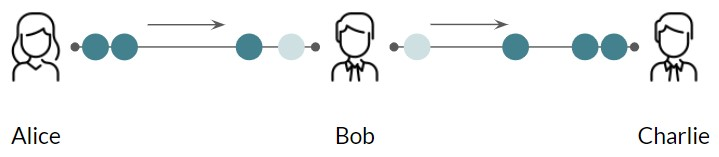
\includegraphics[width=12cm]{07_Beads}
	\caption{Alice can pay Charlie through Bob by paying Bob first and then letting Bob pay Charlie}
	\label{fig:07_Beads}
\end{figure}

\section{Hash and Timelock Contracts}
\par The concept of routed payments provides an excellent contribution to the efficiency of the Lightning Network.

\chapter{Protential Risks of the Lightning Network}
\section{Coin Theft via Tracking}

\chapter{Use Cases}
\section{Instant Payment in a Coffee Shop}
\section{Micropayments for Internet Service}
\section{Routed Payments}

\end{document}
